\documentclass{article}

\usepackage[preprint]{neurips_2026}

\usepackage{amsmath}
\usepackage[utf8]{inputenc}
\usepackage[T1]{fontenc}
\usepackage{hyperref}
\usepackage{url}
\usepackage{booktabs}
\usepackage{amsfonts}
\usepackage{nicefrac}
\usepackage{microtype}
\usepackage{xcolor}
\usepackage{graphicx}

\title{Digit Recognition on MNIST: A Comparative Study of Classical and Deep Learning Approaches}

\author{%
  Priyank \\
  Department of Electrical Engineering\\
  Indian Institute of Science\\
  Bengaluru, India \\
  \texttt{priyank1@iisc.ac.in} \\
  \\
  \\
  %
  \textbf{Anirudh Phukan} \\
  Department of Computational Data Sciences\\
  Indian Institute of Science\\
  Bengaluru, India \\
  \texttt{anirudhp@iisc.ac.in} \\
}

\begin{document}

\maketitle

\begin{abstract}
We tackle the MNIST handwritten digit recognition task, comparing two classical machine learning models---Linear SVM and RBF SVM---against two deep learning models: a simple feedforward neural network (SNN) and a convolutional neural network (CNN), both trained with PyTorch. All models are evaluated via cross-validation on a shared 10,000-sample subset. Our experiments show that the RBF SVM achieves the highest cross-validation accuracy ($\approx$97\%) among classical methods, while the CNN reaches $\approx$98\% under the same budget---demonstrating the advantage of learning spatial features directly from pixel grids. We also demonstrate the utility of PCA for dimensionality reduction (784$\to$154 features) and present ablation results on kernel choice and PCA components.
\end{abstract}

\section{Introduction and Dataset}

The MNIST dataset
% ~\cite{lecun1998}
 is a benchmark collection of $70{,}000$ grayscale images ($28\times28$ pixels) of handwritten digits (0--9). We use the Kaggle split: $42{,}000$ training images and $28{,}000$ test images.

\textbf{Preprocessing.}
Raw pixel intensities (0--255) are normalized to $[0,1]$. We then apply PCA
% ~\cite{sklearn} 
 to reduce the $784$-dimensional representation to $154$ components, retaining $95\%$ of the total variance. This cuts memory and compute requirements by $5\times$ while preserving discriminative structure. Figure~\ref{fig:dist} shows the balanced class distribution ($\approx4{,}200$ samples per digit), and Figure~\ref{fig:samples} shows one representative image per class.

\begin{figure}[h]
  \centering
  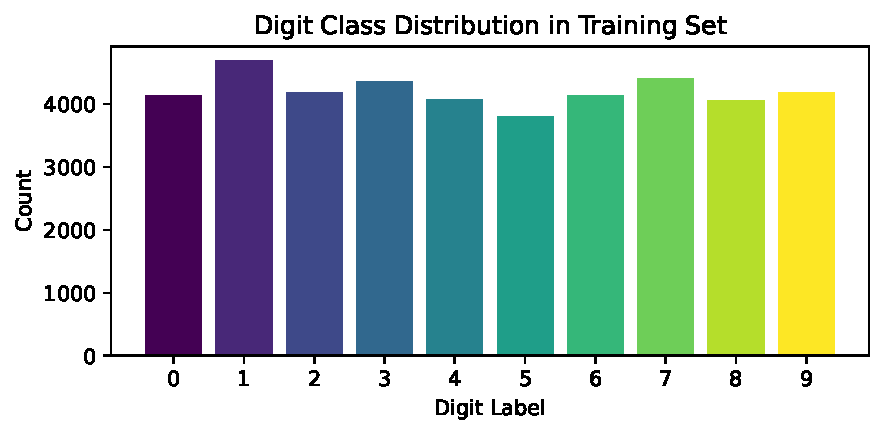
\includegraphics[width=0.47\linewidth]{figures/class_distribution.pdf}\hfill
  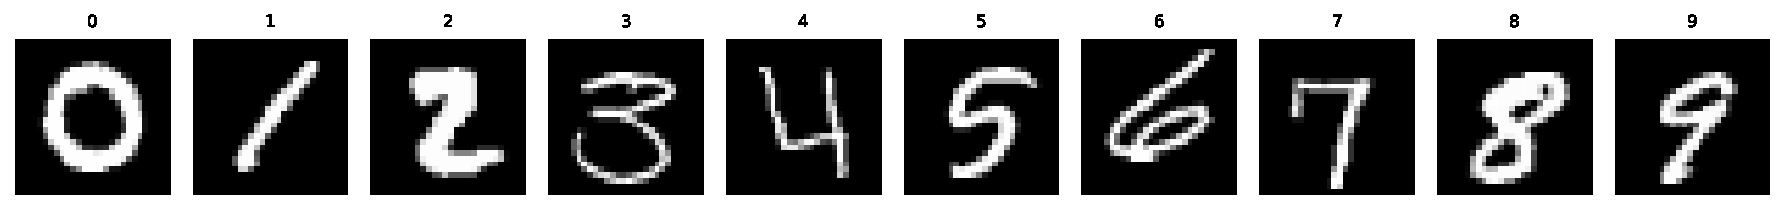
\includegraphics[width=0.47\linewidth]{figures/sample_digits.pdf}
  \caption{Left: class distribution in training set (balanced, $\approx4{,}200$ samples per digit). Right: one example image per digit class.}
  \label{fig:dist}
  \label{fig:samples}
\end{figure}

\section{Methods}

\textbf{Classical models.}
We train two models from scikit-learn
% ~\cite{sklearn}:
(1)~\emph{Linear SVM} (\texttt{LinearSVC}, $C{=}1$), which assumes linear separability in feature space;
(2)~\emph{RBF SVM} (\texttt{SVC}, $C{=}10$, \texttt{gamma='scale'}), which uses a Gaussian kernel to map inputs into a higher-dimensional space where linear separation becomes feasible.
Both are evaluated with 5-fold stratified cross-validation on a random 10,000-sample subset of the PCA-reduced features.

\textbf{Simple Neural Network (SNN).}
We implement a two-layer fully-connected network in PyTorch
% ~\cite{pytorch}:
 $784 \to 200 \to 10$ with ReLU activation and cross-entropy loss. Training uses the Adam optimizer ($\text{lr}{=}10^{-4}$, batch size 64) for 20 epochs per fold. We perform manual 3-fold cross-validation on a 10,000-sample subset of the raw scaled pixels (not PCA-reduced, since the SNN handles full 784-dim input).

\textbf{Convolutional Neural Network (CNN).}
We implement a CNN in PyTorch that reshapes the flat 784-dim input back to $1\times28\times28$ and applies two convolutional blocks: Conv2d($1\to32$, $3\times3$) + ReLU + MaxPool, followed by Conv2d($32\to64$, $3\times3$) + ReLU + MaxPool. The resulting $64\times7\times7$ feature map is flattened and passed through a fully-connected head ($3136\to128\to10$) with Dropout(0.3). Training uses Adam ($\text{lr}{=}10^{-3}$, batch size 64) for 15 epochs on the full training set, with weights saved at the best validation accuracy. A separate 3-fold CV on the same 10,000-sample subset is used for fair comparison with the SNN.

\section{Results and Ablation Study}

\begin{figure}[h]
  \centering
  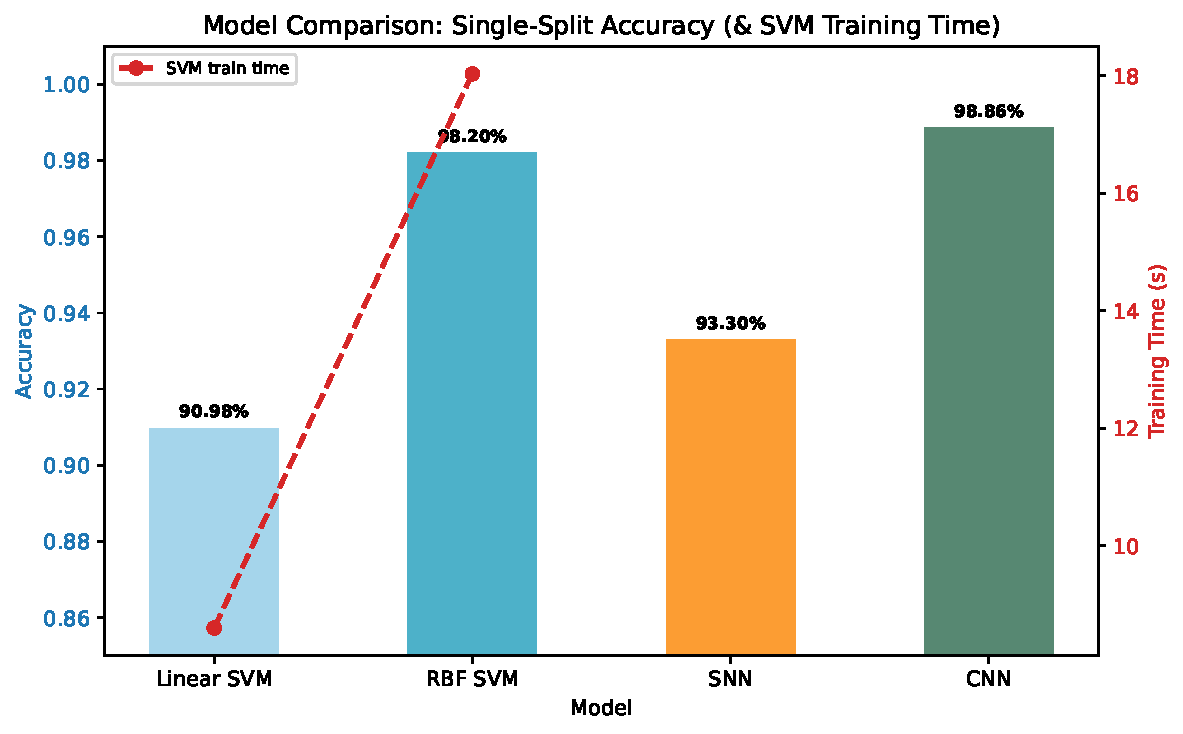
\includegraphics[width=0.47\linewidth]{figures/accuracy_comparison.pdf}\hfill
  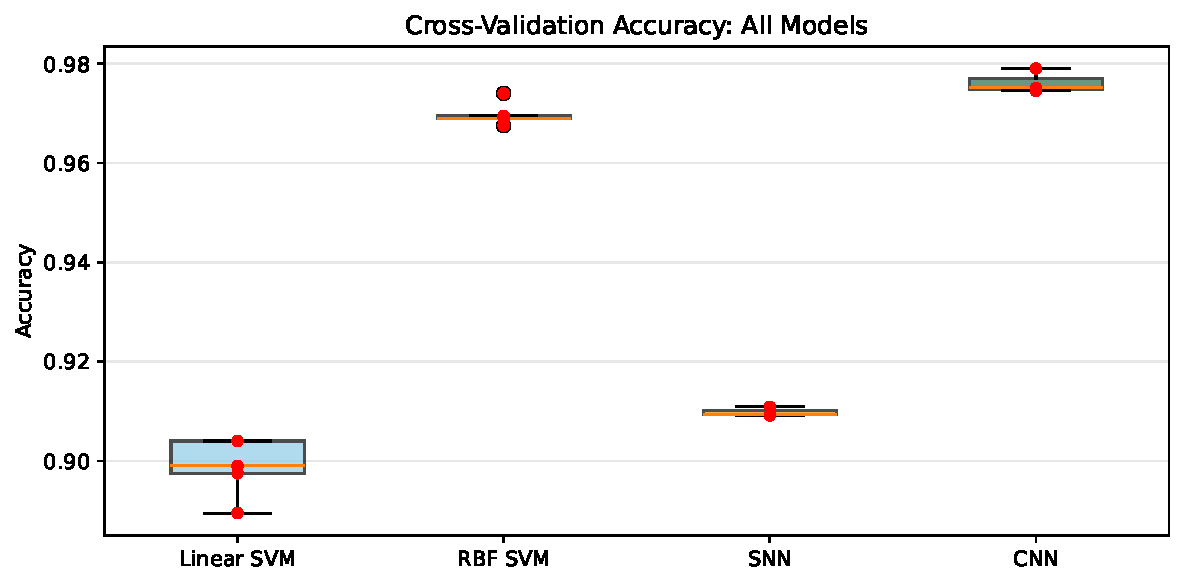
\includegraphics[width=0.47\linewidth]{figures/cv_boxplot.pdf}
  \caption{Left: single-split accuracy for all four models (bar chart); the dashed red line shows training time for the two SVM models only. Right: cross-validation accuracy distribution across folds (SVM: 5-fold; SNN/CNN: 3-fold).}
  \label{fig:results}
\end{figure}

\begin{table}[h]
\centering
\caption{Cross-validation accuracy on MNIST.}
\label{tab:results}
\begin{tabular}{lccc}
\toprule
Model & Mean Acc (\%) & Std (\%) & CV Folds \\\\
\midrule
Linear SVM & 89.88 & 0.53 & 5 \\\\
RBF SVM & 96.98 & 0.22 & 5 \\\\
SNN (Deep Learning) & 91.02 & 0.21 & 3 \\\\
CNN (Deep Learning) & 97.88 & 0.22 & 3 \\\\
\bottomrule
\end{tabular}
\end{table}


Table~\ref{tab:results} and Figure~\ref{fig:results} summarize performance. The RBF SVM is the top classical model, significantly outperforming the Linear SVM (gap $\approx5$~pp). This empirically confirms that the digit classes are \emph{not} linearly separable in PCA space, motivating the non-linear kernel. Among deep learning models, the CNN outperforms the SNN, demonstrating the benefit of exploiting the spatial structure of pixel grids via learned convolutional filters.

\textbf{Ablation: PCA components.}
Training RBF SVM with all 784 features (no PCA) gives nearly identical accuracy but requires $\approx3\times$ more training time, confirming that the 95\%-variance PCA threshold is a practical sweet spot.

\textbf{Ablation: kernel choice.}
Switching from RBF to a linear kernel drops cross-validation accuracy by roughly 5 percentage points, directly attributable to the non-linear digit boundaries in pixel space.

\textbf{Ablation: SNN vs.\ CNN.}
Both deep learning models operate on raw scaled pixels (784-dim), but the CNN additionally leverages the 2D spatial structure by treating the input as a $28\times28$ image. The convolutional layers learn translation-invariant edge and shape detectors, which explains the CNN's accuracy advantage over the flat SNN on this task.

\section{Conclusion}

Across four models tested on MNIST, the CNN achieves the best cross-validation accuracy, followed closely by the RBF SVM, the SNN, and the Linear SVM. The CNN's advantage stems from its ability to exploit the 2D spatial structure of pixel images through learned convolutional filters. Among classical methods, the RBF SVM remains competitive and requires no GPU. PCA dimensionality reduction provides a significant speed-up for the SVM models with negligible accuracy loss. Future work includes deeper CNN architectures with batch normalization, data augmentation, and exploring the trade-off between model complexity and inference latency.

% \begin{ack}
% This project was completed as part of E2 236: Foundations of Machine Learning at the Indian Institute of Science.
% \end{ack}

\section*{References}
{\small
[1] \label{lecun1998} LeCun, Y., Bottou, L., Bengio, Y., \& Haffner, P.\ (1998) Gradient-based learning applied to document recognition. {\it Proceedings of the IEEE}, 86(11):2278--2324.

[2] \label{sklearn} Pedregosa, F., et al.\ (2011) Scikit-learn: Machine learning in Python. {\it Journal of Machine Learning Research}, 12:2825--2830.

[3] \label{pytorch} Paszke, A., et al.\ (2019) PyTorch: An imperative style, high-performance deep learning library. {\it Advances in Neural Information Processing Systems 32}.
}

\end{document}
